\def \digital{1}
\if 1\digital
	\documentclass[12pt]{report}
\else
	\documentclass[twoside,openright,12pt]{report}
\fi

\usepackage[no-math]{fontspec}
\usepackage{amsmath}
\usepackage{amssymb}
\usepackage{xltxtra}
% \usepackage{xgreek}
% 	\nogreekalph

\usepackage{newtxmath}
\setmainfont{Times New Roman}
\setmonofont[Scale=MatchLowercase]{SourceCodePro-Regular.otf}

\usepackage{geometry}
\geometry{
	a4paper,
	headheight= 14.5pt,
	left=2.54cm,
	right=2.54cm,
	top=2.54cm,
	bottom=2.54cm
}
\usepackage{fancyhdr}
\usepackage{emptypage}
\usepackage{graphicx}
\graphicspath{ {images/}{plots/} }
\usepackage{hyperref}
\hypersetup{colorlinks,
	citecolor=black,
	filecolor=black,
	linkcolor=black,
	urlcolor=black}

\usepackage[nottoc,notlof,notlot,numbib]{tocbibind}
\usepackage{appendix}
\usepackage{setspace}
\usepackage{multicol}
\usepackage[format=hang,font=normalsize]{caption}
\usepackage{subcaption}
\usepackage[mode=text]{siunitx}
\usepackage{standalone}
\usepackage{float}
\usepackage{parskip}
\usepackage{listings}
\usepackage[toc]{glossaries}
\usepackage{listings-golang} % import this package after listings

\usepackage{lstautogobble}  % Fix relative indenting
\usepackage{color}          % Code coloring
\usepackage{zi4}            % Nice font

\definecolor{bluekeywords}{rgb}{0.13, 0.13, 1}
\definecolor{greencomments}{rgb}{0, 0.5, 0}
\definecolor{redstrings}{rgb}{0.9, 0, 0}
\definecolor{graynumbers}{rgb}{0.5, 0.5, 0.5}

\lstset{ 
    numbers=left,
    numbersep=15pt,
    autogobble,
    columns=fullflexible,
    showspaces=false,
    showtabs=false,
    breaklines=true,
    showstringspaces=false,
    breakatwhitespace=true,
    escapeinside={(*@}{@*)},
    commentstyle=\color{greencomments},
    keywordstyle=\color{bluekeywords},
    stringstyle=\color{redstrings},
    numberstyle=\color{graynumbers},
    basicstyle=\ttfamily\footnotesize,
    frame=l,
    framesep=12pt,
    xleftmargin=12pt,
    tabsize=4,
    captionpos=b,
    language=Golang
}

\newcommand{\blankpage}{
	\newpage
	\thispagestyle{plain}
	\mbox{}
	\newpage
}

\makeglossaries
% \newglossaryentry{ledger}
% {
%     name=ledger,
%     description={A ledger is a shared data structure where one can only read or append records}
% }

% \newglossaryentry{mqtt}{
%     name = MQTT,
%     description = {Message Queuing Telemetry Transport, a lightweight messaging protocol on top of TCP/IP, stands for Message Queuing Telemetry Transport}
% }

% \newglossaryentry{utxo}{
%     name = UTXO,
%     description = {Unspent transaction output, a record keeping model, they work like paper bills which means you need to consume the whole bill to make a transaction and you get change back (another UTXO)}
% }

% \newglossaryentry{pow}{
%     name = PoW,
%     description = {Proof of Work, a consensus algorithm that decides which node's block will be added to the blockchain}
% }

% \newglossaryentry{DDoS}{
%     name = DDoS,
%     description = {Distributed Denial of Service, a networking attack where the adversary tries to halt services by flooding a server with multiple requests}
% }

\newacronym{hlf}{HLF}{Hyperledger Fabric}
\newacronym{dlt}{DLT}{Distributed Ledger Technology}
\newacronym{iot}{IoT}{Internet of Things}
\newacronym{iiot}{IIoT}{Industrial Internet of Things}
\newacronym{btc}{BTC}{Bitcoin's currency}
\newacronym{eth}{ETH}{Ethereum's native currency}
\newacronym{b2b}{B2B}{Business to Business}
\newacronym{b2b2c}{B2B2C}{Business to Business to Customer}
\newacronym{txp}{TXP}{Transaction Proposal}
\newacronym{txpr}{TXPR}{Transaction Proposal Response}
\newacronym{p2p}{P2P}{peer-to-peer}
\newacronym{ble}{BLE}{Bluetooth low energy}
\newacronym{hsm}{HSM}{Hardware Security Module}
\newacronym{tee}{TEE}{Trusted Execution Environment}
\newacronym{m2m}{M2M}{machine-to-machine}
\newacronym{pki}{PKI}{Public Key Infrastructure}
\newacronym{evm}{EVM}{Ethereum Virtual Machine}
\newacronym{msp}{MSP}{Membership Service Provider}
\newacronym{ddos}{DDoS}{Distributed Denial of Service}
\newacronym{sdk}{SDK}{Standard Development Kit}
\newacronym{ca}{CA}{Certificate Authority}
\newacronym{pow}{PoW}{Proof of Work}
\newacronym{pos}{PoS}{Proof of Stake}
\newacronym{bft}{BFT}{Byzantine Fault Tolerance}
\newacronym{utxo}{UTXO}{Unspent Transaction Output}
\newacronym{mqtt}{MQTT}{Message Queuing Telemetry Transport}
\newacronym{mcu}{MCU}{Microcontroller Unit}
\newacronym{eoa}{EOA}{Externally Owned Accounts}

\def\bitcoin{%
  \leavevmode
  \vtop{\offinterlineskip %\bfseries
    \setbox0=\hbox{B}%
    \setbox2=\hbox to\wd0{\hfil\hskip-.03em
    \vrule height .3ex width .15ex\hskip .08em
    \vrule height .3ex width .15ex\hfil}
    \vbox{\copy2\box0}\box2}}

\begin{document}
\pagenumbering{roman}

\begin{titlepage}
	\centering
	{\scshape\Large Aristotle University of Thessaloniki \par}
	{\scshape\Large Faculty of Engineering \par}
    {\scshape\Large School of Electrical \& Computer Engineering \par}
% 	{\scshape\Large Department of Electronics \& Computers  \par}
	\vspace{0.5cm}
	\includegraphics[width=0.25\textwidth]{LogoAUTHblack} \par
	\vspace{1cm}
	{\scshape In collaboration with \par}
	\label{r}
	{\scshape\large IBM Research Zürich \& IBM CIC Benelux \par}
	\vspace{0.5cm}
	{\scshape\Large Diploma Thesis \par}
%	\hrulefill \par
	\vspace{0.3cm}
	{\huge\bfseries Towards low-powered Industrial IoT devices transacting with consortium blockchains\par} 
	% alternative title:  A lightweight SDK for low power IoT devices to transact with a Hyperledger Fabric Network 
	% Can consortium blockchains be used for IoT?
	\vspace{2cm}
	{\Large\itshape Amoutzias Athanasios \par}
	\vfill
	{\scshape\large Supervisor \par}
	{\large Dimitrios Mitrakos \par}
	{\large \textit{Associate Professor}}
	\vfill
% % 	{\scshape\large - \par}
% 	{\large } 
% 	{\large }
	
	\vfill
	{\scshape\large Thessaloniki, March 2019\par}
\end{titlepage}

\if 1\digital
	\newgeometry{
		headheight= 14.5pt,
		left=3.1cm,
		right=3.1cm,
		top=2.54cm,
		bottom=2.54cm
	}
\else
	\newgeometry{
		headheight= 14.5pt,
		left=3.6cm,
		right=2.6cm,
		top=2.54cm,
		bottom=2.54cm
	}
\fi

\pagestyle{fancy}
\fancyhf{}
\fancyhead[L]{\textit{ \nouppercase{\leftmark}} }
\fancyhead[R]{\textit{ \nouppercase{\rightmark}} }
\if 1\digital
	\fancyfoot[C]{\thepage}
	\fancypagestyle{plain}{
		\fancyhf{}
		\renewcommand{\headrulewidth}{0pt}
		\renewcommand{\footrulewidth}{0pt}
		\fancyfoot[C]{\thepage}
	}
	\fancypagestyle{empty}{
		\fancyhf{}
		\renewcommand{\headrulewidth}{0pt}
		\renewcommand{\footrulewidth}{0pt}
		\fancyfoot[C]{\thepage}
	}
\else
	\fancyfoot[LE,RO]{\thepage}
	\fancypagestyle{plain}{
		\fancyhf{}
		\renewcommand{\headrulewidth}{0pt}
		\renewcommand{\footrulewidth}{0pt}
		\fancyfoot[LE,RO]{\thepage}
	}
	\fancypagestyle{empty}{
		\fancyhf{}
		\renewcommand{\headrulewidth}{0pt}
		\renewcommand{\footrulewidth}{0pt}
		\fancyfoot[LE,RO]{\thepage}
	}
\fi

\setcounter{page}{2}
%====================intro chapters=============================
\chapter*{}
\thispagestyle{plain} \null
\vfill
 \vspace{0.25cm}
	\includegraphics[width=0.5\textwidth]{Pale_Blue_Dot.png}\par
	\vspace{1cm}
	
\begin{flushright}
Look again at that dot. That's here. That's home. That's us. On it everyone you love, everyone you know, everyone you ever heard of, every human being who ever was, lived out their lives. The aggregate of our joy and suffering, thousands of confident religions, ideologies, and economic doctrines, every hunter and forager, every hero and coward, every creator and destroyer of civilization, every king and peasant, every young couple in love, every mother and father, hopeful child, inventor and explorer, every teacher of morals, every corrupt politician, every "superstar," every "supreme leader," every saint and sinner in the history of our species lived there-on a mote of dust suspended in a sunbeam.

	\textit{Carl Sagan}
	\par\medskip
\end{flushright}
\vfill\vfill
\chapter*{Acknowledgements}
Foremost, I would like to express my sincere gratitude to my thesis advisor Associate Professor Dimitrios Mitrakos. Firstly, for giving me the freedom and guidance to work on a fairly new and unexplored topic, and secondly for his openness and patience. Besides my advisor, I would also like to thank my mentor during my internship at IBM, Luigi Venti, for his support, guidance and ideas. My grateful thanks are also extended to Dr. Gero Dittmann and Dr. Jens Jelitto from IBM Research Zurich for our collaboration on performance analysis on their project. Additionally, I would also like to show my appreciation to Arne Rutjes for his ideas, connections, knowledge and genuine interest on the subject as well as to all my colleagues who contributed with their ideas, open discussions and suggestions. Furthermore, I wish to express my gratitude to the IBM CIC Benelux for giving me the opportunity to do research, collaborate and write this thesis as well as to Ieremias Athanasiadis for introducing me to the group.

Finally, I want to thank my friends and peers for all their crucial support during difficult moments and for inspiring me throughout my studies with their exquisite work and contributions.

Ultimately, I want to express my deepest gratitude to my family, my brother for his crucial help and especially my mother, who unquestionably supported and encouraged me throughout my life.
\chapter*{Abstract}
%https://www.scribbr.com/dissertation/abstract/

% With the invention of Bitcoin and the emergence of blockchain platforms, consortium blockchain networks came to existence. Hyperledger Fabric is such a tool to provide businesses with permissioned blockchain networks and accelerate their workflows. Additionally, business and the industry use \acrshort{iot} devices for automation, control, tracking and monitoring, but being in their early stage they introduce a notable attack surface \cite{secure-IoT}. In this thesis, we investigate the applicability of blockchains on \acrshort{iot} and we introduce a lightweight SDK, developed by Dr. Gero Dittmann \cite{gero} and Dr. Jens Jelitto \cite{jens} from IBM Zurich, to enable devices transact with a Hyperledger Fabric Network. Finally, we conclude with an analysis of the SDK with respect to performance.

% In this thesis we built the fundamentals of blockchains starting from the origin, Bitcoin. We continue with Ethereum and how it expanded on Bitcoin.  We proceed with introducing \acrlong{hlf}, an adaptation of blockchain as an idea and a network to help accelerate transactions between parties. 

% Our research question formulates around the applicability of blockchain on internet of things and 


%Problem statement
%The first sentence establishes the topic and main problem that the research will address. This problem will lead to the objective and research questions.

% Environmental non-profit organizations in the UK currently face a significant funding gap. 
With the invention of Bitcoin and the emergence of blockchain platforms, consortium blockchain networks came to existence. \acrlong{hlf} is a tool to provide businesses with permissioned blockchain networks and accelerate their workflows. Additionally, industry  uses \acrlong{iot} devices for automation, controlling, tracking and monitoring, but being in their early stage they introduce a notable attack surface \cite{secure-IoT} and they suffer from standardization. Research has shown that blockchains can be effective on the security of \acrshort{iot} devices as well as offer a common platform to create standards. This study aims to bridge \acrshort{iot} and permissioned blockchain setups with \acrlong{hlf} and provide a performance analysis of a tool\footnote{developed by Dr. Gero Dittmann \cite{gero} and Dr. Jens Jelitto \cite{jens} from IBM Zurich} that enables low-powered devices to transact with a blockchain network. Building on existing work on the applicability of \acrshort{iot} and blockchains, it asks: How can a low-powered device transact with a \acrlong{hlf} network, what are the benefits, how does it perform, can it scale down further and open the doors to microcontrollers? In this context, consortium or permissioned blockchains are defined as networks that connect known entities which collaborate and/or have competing interests.

Our approach is based on a review of literature on permissioned blockchains, IoT security, use cases and finally a performance analysis of a tool that bridges \acrshort{iot} and \acrlong{hlf}. Indeed blockchains can strengthen the security and automation of \acrshort{iot} and can be seen as a provider of trust for transacting devices. Performance analysis demonstrated an improvement of 71\% on bandwidth usage and 53\% on CPU resources, thus establishing the first step to scale down further.

% Background 
% There is a brief summary of the scholarly context to show the study's relevance.

%Research has shown that donation intention is influenced by campaign messaging strategies, and that representations of individual victims are generally more effective than appeals based on abstract concepts like climate change.



%Objective
%Next, the specific objective of the research is stated.
% This study aims to determine how environmental organizations can target fundraising campaigns to increase donations. 

% This study aims to bridge \acrshort{iot} and permissioned blockchain setups with \acrlong{hlf} and provide a performance analysis on a tool\footnote{developed by Dr. Gero Dittmann \cite{gero} and Dr. Jens Jelitto \cite{jens} from IBM Zurich} that enables low-powered devices to transact with a blockchain network.

%Research question
%The topic is narrowed down even further in the main research question, which shows exactly what the study aims to find out.

%Building on existing work on targeted fundraising, it asks: To what extent does a potential donor's social distance from climate change victims in fundraising campaigns affect their intention to make a donation?

% Building on existing work on the applicability of \acrshort{iot} and blockchains, it asks: How can a low-power device transact with a \acrshort{hlf} network, what are the benefits, how does it perform, can it further scale down and open the doors to \acrshort{mcu}s?

%Definition 
%If your abstract uses specialized terms that would be unfamiliar to the average academic reader or that have various different meanings, give a concise definition.
%In this context, social distance is defined as the extent to which people feel they are in the same social group (in-group) or another social group (out-group) in relation to climate change victims.

% In this context, consortium or permissioned blockchains are defined as networks that connect known entities that collaborate and/or have competing interests.
%----

%Methodology
%The next step is a brief description of the methods used to answer the research question.
%Based on a review of the literature on donation intention and theories of social distance, an online survey was distributed to potential donors based across the UK. Respondents were randomly divided into two conditions (large and small social distance) and asked to respond to one of two sets of fundraising material. 

% Our approach is based on a review of literature on permissioned blockchains, IoT security, use cases and finally a performance analysis of a tool that bridges \acrshort{iot} and \acrshort{hlf}. 

%Results
%The most important results are summarized.
%Analysis of the responses demonstrated that large social distance was associated with stronger donation intentions than small social distance.
% Indeed blockchains can strengthen the security and automation of \acrshort{iot} and can be seen as a provider of trust for transacting devices. Performance analysis demonstrated an improvement of 71\% on bandwidth usage and 53\% on CPU resources, thus establishing the first step to scale down further.

%Conclusions
%Finally, the study's main conclusions are stated, directly answering the research question and objective. As this research focused on a practical problem, it also includes recommendations.
%The results indicate that social distance does have an impact on donation intention. On this basis, it is recommended that environmental organizations use social distance as a key factor in designing and targeting their campaigns. Further research is needed to identify other factors that could strengthen the effectiveness of these campaigns.
%===============================================================
\tableofcontents 
\thispagestyle{plain}
\listoffigures
\thispagestyle{plain}
\listoftables
\setglossarystyle{listhypergroup}
%for hyperlinking terms on text and sort them alphabetically
\printglossaries
\if 1\digital
\newgeometry{
	headheight= 14.5pt,
	%left=3.18cm,
	left=3.81cm,
	right=3.18cm,
	top=2.54cm,
	bottom=2.54cm
}
\else
\newgeometry{
	headheight= 14.5pt,
	left=3.68cm,
	right=2.68cm,
	top=2.54cm,
	bottom=2.54cm
}
\fi
%===========================chapters============================
\chapter{Introduction}
\pagenumbering{arabic}

\section{Motivation} %needs integration between the work done, the need for industry and the history of blockchains

In 2008, Satoshi Nakamoto published the Bitcoin whitepaper\cite{nakamoto2008bitcoin} where he described a decentralized network that enabled electronic currency with some very peculiar characteristics. The main achievement of this network, that came into existence in early 2009, is that it solves the double spending problem by making everyone's best economic interest to support an honest network. Blockchain as cryptographically linking blocks in an append-only data structure existed long before the introduction of Bitcoin \cite{haber1990time}. Young Vitalik Buterin, inspired by the work of Satoshi Nakamoto and already contributing to the Bitcoin codebase published the whitepaper of Ethereum \cite{buterin2013ethereum}. Ethereum is a Turing complete solution contradicting to Bitcoin. With the rise of Turing complete blockchain networks, consortium blockchains came to existence. We are investigating one of the Hyperledger frameworks, the \acrlong{hlf} \cite{androulaki2018hyperledger}. Fundamentally it is a \acrfull{dlt}, which means a shared ledger in a permissioned network with competing interest players. Consortium blockchains or \acrshort{dlt}s are created to accelerate \acrshort{b2b} and \acrshort{b2b2c} interactions, at their base they are centralized-authoritarian, distributed databases, recorded in a blockchain fashion, with transaction based signed messages. 

With the surge of \acrfull{iot} devices in consumer products and in the industry the attack surface has increased and security breaches have risen \cite{gemalto-iot}. Thus, under some circumstances, distributed ledgers can be a suitable solution to mitigate specific attacks and accelerate the current workflow. We believe, it is always important to have the right tools for the job and make them easily accessible to everyone.

\section{Research Topics}
We aim to explore the following research topics in this thesis:

1. Consortium Blockchains and applications.

2. Integration of Internet of Things and Blockchains.

3. Identity of things and trusted operations.

% \section{Scope}
% This study focuses on making trustless IoT devices by enabling them to transact with a consortium blockchain, \acrfull{hlf}.

% We start by covering some basic background around blockchains while explaining Bitcoin and Ethereum. We continue by examining the transaction flow of Hyperledger Fabric and we suggest, then implement a solution to abstract it and make it available for low-powered IoT devices.

\section{Outline}
% We start at chapter 2 with an introduction to cryptographical hash functions, asymmetric cryptography and \acrfull{pki}. We continue with Bitcoin and how transactions take place and consensus is reached, we expand with Ethereum and finally make an abstraction of blockchain attributes, summarizing the key characteristics of a permissionless blockchain network. 

We start at chapter 2 with an introduction to cryptographical hash functions, asymmetric cryptography and \acrfull{pki}. We continue with Bitcoin and how transactions take place and consensus is reached and we expand on Ethereum. 

In chapter 3 we discuss about the adoption, mutation of blockchains in the industry and how they differ from public networks. We continue with Internet of Things in industry and finally we conclude by merging both topics with a case study.

In chapter 4 we dive in \acrlong{hlf}, our tool of choice. We elaborate on transactions, smart contracts and key components of this network. 

In chapter 5 we present related work done with \acrshort{iot} and blockchains, what other companies do, what academia researches, what IBM does and how we expand on that.

In chapter 6 we offer an analysis of a new tool while providing a brief background on software profiling. 

In chapter 7 we conclude and discuss about future work.
\chapter{Blockchain Essentials}
We cover the fundamentals needed to explain blockchain networks. At the first section, we start by covering fundamental cryptography concepts, next we cover the origin of blockchains; Bitcoin and how it works, then we continue with Ethereum and how it expanded and diverged from Bitcoin.
% and finally we abstract and summarize the attributes of blockchains.

\section{General Background}
This section covers basic cryptographic concepts that run the web of trust today.

\subsection{Cryptographic Hash Functions}
A cryptographic hash function is a computationally efficient mathematical algorithm, that has certain properties which make it suitable for cryptography. It maps data of arbitrary size to a bit string of fixed size, known as hash. The slightest change to the input makes a large change in the resulting hash. Designed to be a one-way function, it is easy to produce the output given the input but computationally infeasible to produce the input given the output. In theoretical cryptography, the security level of a cryptographic hash function has been defined using the following properties. \footnote{$H$ is a hash function with inputs $x,x'$ and outputs $y,y'$} \cite{katz1996handbook}

\begin{enumerate} 
    \item \textbf{Preimage resistance}: It is computationally infeasible to find any input $x$ which hashes to that output $y$. Given $y$, it is difficult to find any preimage $x'$ such that $H(x')=y$ when given any $y$ for which the corresponding input $x$ is not known. 
    \item \textbf{Second preimage resistance}: It is computationally infeasible to find any second input which has the same output as any specified input, that is given $x$ to find a 2nd-preimage $x'\neq x$ such that $H(x)=H(x')$.
    \item \textbf{Collision Resistance}: It is computationally infeasible to find any two distinct inputs $x,x'$ which hash to the same output such that $H(x)=H(x')$
\end{enumerate}
\subsection{Public Key Cryptography}
\acrfull{pki} also referred to as asymmetric cryptography, is a system that uses a pair of keys, a \textit{public key} $e$ that is widely known and a corresponding \textit{private key} $d$ which is known only to the owner. The two keys have a mathematical relationship and in secure systems the task of computing $d$ given $e$ is computationally infeasible. In such a system, any person can encrypt a message using the receiver's \textit{public key} and that encrypted message can only be decrypted by the receiver's \textit{private key}. The public key defines an \textit{encryption transformation} $E_e$, while the private key defines the associated \textit{decryption transformation} $D_d$. Any entity $B$ wishing to send a message $m$ to $A$ obtains $A$'s public key $e$, uses the encryption transformation to obtain the \textit{ciphertext} $c=E_e(m)$ and transmits $c$ to $A$. To decrypt $c$, $A$ applies the decryption transformation to obtain the original message $m=D_d(c)$

% How do we achieve integrity and non repudiation with public key cryptography?
Public key cryptography establishes a secure communication by satisfying the following cryptographic objectives:
\begin{enumerate}
    \item \textbf{Confidentiality}: Keeps the content of information from all but those authorized to have it. Achieved by encrypting, $B$ uses $A$'s public key to encrypt the message and only $B$ can decrypt that message with its private key, but anyone could impersonate $A$.
    \item \textbf{Data Integrity}: Addresses the unauthorized alteration of data using digital signatures. Digital signatures is a scheme where both parties verify that the information sent was created by the claimed sender and has not been tampered with. Entity $A$ uses its private key to produce a hash of the message and attaches it as a signature to the message. Entity $B$ receives the signed message and uses the same hash algorithm that $A$ used with its public key. Finally it compares the resulting hash with the message's actual hash, if the two are equal then it knows the author is the one with the possession of the particular private key.
    \item \textbf{Authentication}: Associated with identification and applied to both entities and the data itself, which implicitly provides data integrity. Achieved by encrypting ones message with its own private key, $B$ uses its private key to encrypt the message and send it to $A$, it can decrypt the message using $B$'s public key and thus verifying the sender, but anyone intercepting the communication can decrypt it.
    \item \textbf{Non-repudiation} Prevents an entity from denying actions by using digital signatures, a procedure that involves a trusted third party to resolve the dispute. i.e  $A$ authorizes a transaction to sent an asset to $B$ and later denies it. Since the transaction is signed with $A$'s private key, there is no room questioning.
\end{enumerate}
\begin{figure}[H]
        \centering
        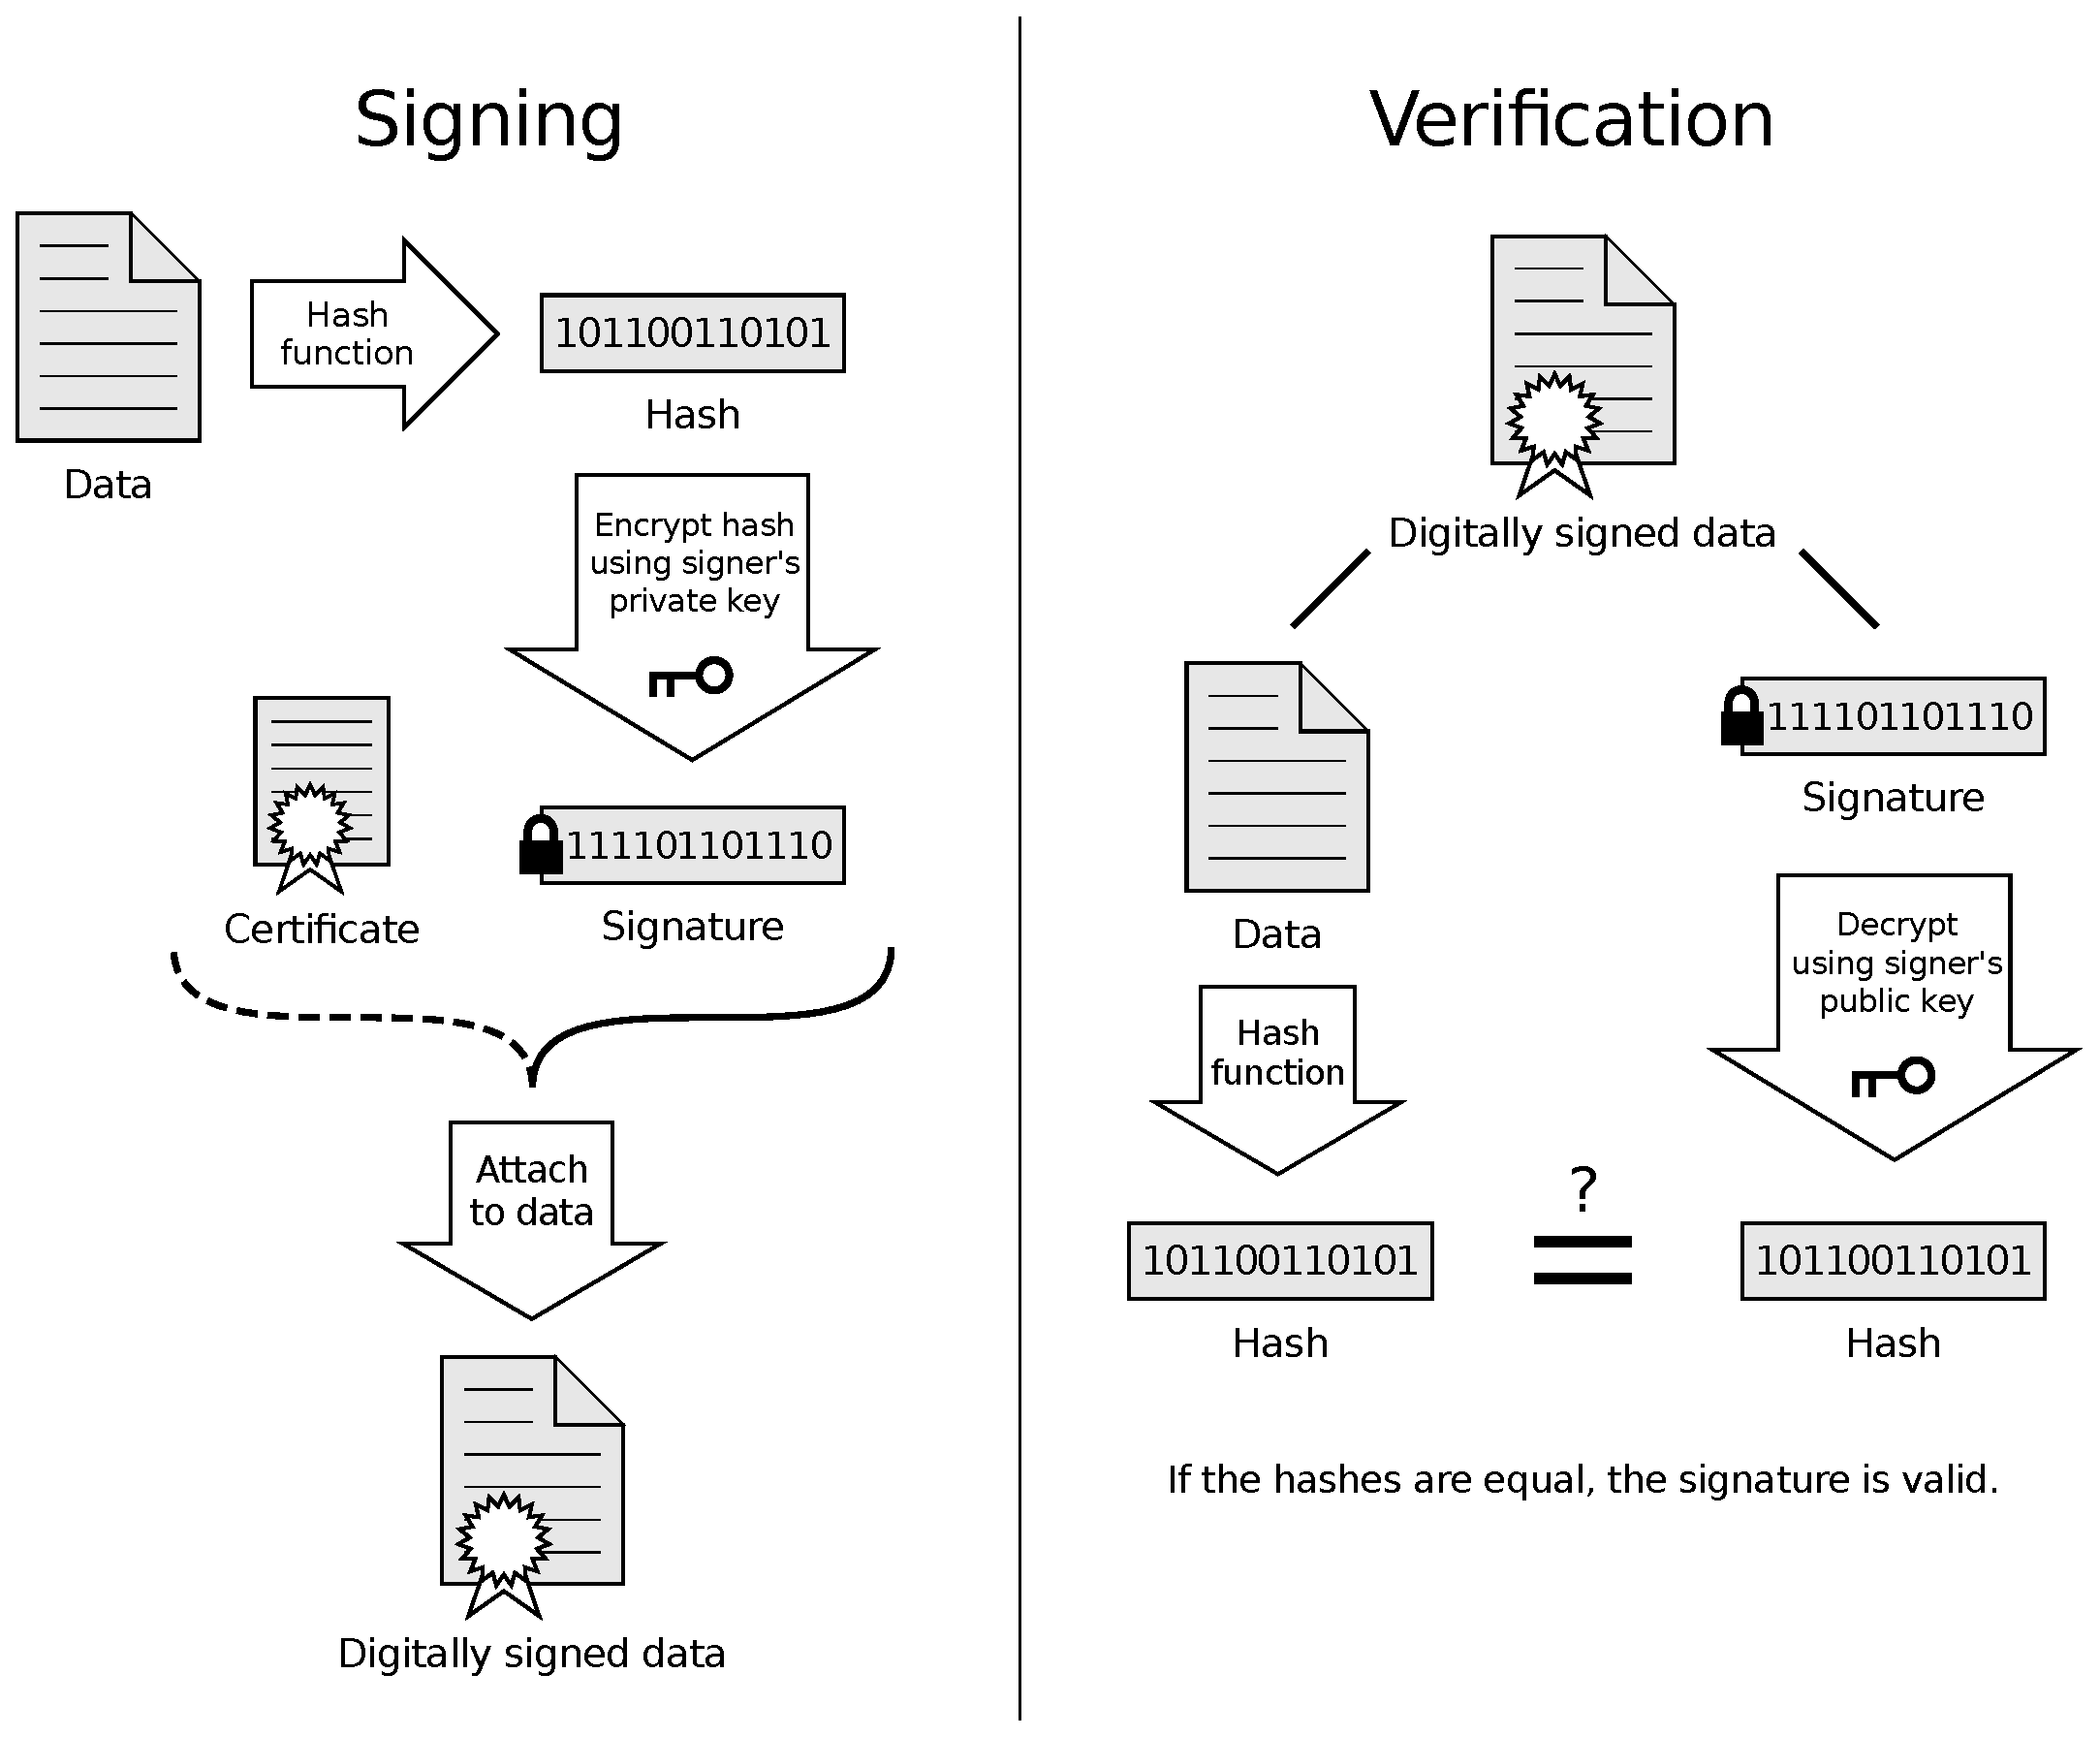
\includegraphics[width=1\textwidth]{Digital_Signature_diagram.eps}
        \caption{How digital signing works \cite{wiki:digital-signature}.}
        \label{fig:dig_sign}
    \end{figure}	
\subsection{Public Key Infrastructure}
In this subsection we cover the basics of Public Key infrastructure in order to associate them later to Fabric's components. 
PKI comprises \cite{CertificatesPKI} :
\begin{itemize}
    \item \textbf{\acrfull{ca}}: A trusted node that acts as a maintainer, keeping the public keys for all nodes. The \acrshort{ca} also bootstraps newly joined nodes in the network by adding their public key to their list, thus only the new node and the \acrshort{ca} need to be configured. 
    \item \textbf{Certificates}: A signed document, as a passport, issued by the \acrshort{ca} stating that a particular name holds a particular private key. Other parties, knowing the public key of \acrshort{ca}, can authenticate a user.  
    \item A repository for retrieving certificates.
    \item A method of revoking certificates.
    \item A method of evaluating a chain of certificates from known public keys to the target name.
\end{itemize}
\section{Bitcoin}
%citations to Mastering Bitcoin, bitcoinwiki, Szabo and Nakamoto
%Transaction flow, mining, cryptoeconomics, network stability, overhead, slow, secure.
% Cryptoeconomics, incentive compatibility through mining fees and BTC minting.
\subsection{Overview}
Bitcoin is a payment network protocol that enables \acrshort{p2p} payments in a sense that no central authority issues new money or tracks transactions. A record of all transactions is held in a shared ledger, where each transaction is verifiable, transparent and can be tracked through all its history. Batches of transactions with a timestamp are called blocks and each block is cryptographically connected to its previous block by including the hash of the previous block. In that manner, a chronological data structure is created, containing verifiable transactions, or else money, that can be spent by the owner's keys. 

Bitcoin's blockchain is secured through repeated computations or else sealed with energy expenditure. The end product is a network that does not need any intermediaries, transactions are made in a \acrshort{p2p} fashion and the blockchain through all this energy expenditure becomes secure and immutable.   


Lets assume that Alice wants to send \bitcoin 7 (bitcoins) to Bob. Alice has already \bitcoin10, she creates a transaction with one input and 2 outputs, one for Bob at \bitcoin7 and one to her address for the change at \bitcoin 2.995 and the rest \bitcoin 0.005 are fees to the miners (today's fees are \bitcoin 0.00005000)\cite{btcfees} to get her transaction into a block. The output for Bob is signed with his public key and the output to her address as change is signed with her private key. After the creation of the transaction, it propagates through nodes in the network, with a gossip protocol, where each node upon receiving it validates it and gossips it to other connected nodes. Finally, it ends up to a node which will include it in the next block that it will successfully mine \cite{btc-wiki-transaction}.

Every node is capable of putting transactions they choose in a block and mine it, but nowadays mining is done collectively and the mining pool chooses the transactions for the next block from the transaction pool \cite{pool-statistics}. Now that there is a block candidate with ordered transactions in it, it is repeatedly hashed by changing an additional value called the nonce. After many changes, a hash is found that is smaller than the difficulty target. A legit block nowadays needs to start with 18 zeros. 

Difficulty adjusts every 2016 blocks and it targets the whole network to produce 2016 blocks every two weeks \cite{difficulty}. An interesting fact is that intervals between finding the next block follow a probability distribution that is memoryless. Block times follow the exponential distribution and the probability of a block \textbf{not} being found in $x$ minutes or longer is: 
\begin{equation}
\label{eq:p(x)}
    p(x) = e^{-(x/10)}
\end{equation}
So that means that finding a block in 10 minutes or less gives as a probability of 0.63, calculating for $x=10$ in \ref{eq:p(x)}. The number of blocks that are expected to be found in a certain time (e.g 2016 per two weeks) follow a Poisson process. The probability of finding $k$ blocks in $T$ minutes is:
\begin{equation}
    P(k,T) = ({\frac{T}{10}})^k \times \frac{e^-({T/10})}{k!}
\end{equation}
So the probability of finding exactly six blocks in an hour would be 0.16 \cite{bowden2018block}.
%https://www.reddit.com/r/btc/comments/6v5ee7/block_times_and_probabilities/

\subsection{Transactions and UTXO}
In this subsection, we elaborate on transactions and the \acrfull{utxo} set.

Transactions are the most important part of every blockchain network, they are the fuel that change the state of the blockchain. At a high level, a transaction is the authorization of a value from the owner to the recipient. Then, the new owner becomes capable of spending this new value by creating a new transaction and transferring ownership of the value. The most common transaction form for bitcoin is a single payment as seen in a simplified\footnote{The difference in the input and output value is the transaction fee.} manner in \ref{fig:btc-tx}. At a lower level, one input contains the digital signature and public key\footnote{The sender's public key is used to verify the digital signature.}, the output to the recipient is signed with recipient's public key.
\begin{figure}[h]
    \centering
    \includegraphics[width=1\textwidth]{images/btc-tx.png}
    \caption{A simplified single transaction with one input and one output.}
    \label{fig:btc-tx}
\end{figure}

The fundamental building block of Bitcoin transactions is the \acrshort{utxo} set. This set, consists of \acrshort{utxo}s that are being used as an input to the next transaction. Each \acrshort{utxo} could be described as an instance of a coin, having any arbitrary value, indivisible, that is going to be spent altogether, destroyed and another new \acrshort{utxo} will take its place. Each \acrshort{utxo} that is consumed as an input to a transaction will create a new one. The relationship of inputs(M) and outputs(N) is $M-N $ where $M,N\geq1$ . Wallets track within the \acrshort{utxo} set, which \acrshort{utxo}s the user's private keys can control, and represents it as a balance. A transaction references previous outputs as new inputs and assigns all inputs to new outputs as seen in \ref{fig:utxo}\footnote{Fees have been excluded for simplicity.}.
\begin{figure}[h]
    \centering
    \includegraphics[width=1\textwidth]{images/utxo.png}
    \caption{\acrshort{utxo}s become input to the next transaction.}
    \label{fig:utxo}
\end{figure}

To conclude with \acrshort{utxo}s, we should emphasize their crucial characteristics. Each \acrshort{utxo} is discrete, indivisible, of arbitrary value, denominated in satoshis\footnote{Satoshi is the smallest unit of bitcoin, \bitcoin$10^{-9}$.} The only way to be spent is to be consumed in their entirety by a transaction.
\subsection{The Blockchain}
In this subsection, we elaborate on the abstract idea of blockchain.

An ever-growing distributed list of records, append only, replicated and shared among the participants of the network (aka distributed ledger). Each block in the chain contains a list of transactions and a hash of the previous block. Blockchain is a log whose records are batched into time-stamped blocks where each block is identified by its hash. By including the hash of the previous block\footnote{The Genesis block, is the first block on the chain and it does not include a reference to a previous block.}, it establishes a link between the blocks, thus creating a block-chain. 
	\begin{figure}[H]
	    \centering
	    \includegraphics[width=1\textwidth]{images/blockchain_simplified.png}
	    \caption{Blockchain simplified}
	    \label{fig:block_simpl}
	\end{figure}
A blockchain can be defined as an immutable shared ledger that holds transactions, maintained within a decentralized and distributed network of mutually non-trusting peers. Every peer maintains their copy of the ledger and is responsible of validating each transaction on it.

\subsection{Mining and immutability}
In this subsection, we discuss how \acrshort{pow} works and makes the blockchain immutable. We should state that mining, \acrshort{pow} and consensus are highly interrelated. 

Abstractly, every node, receives a transaction, verifies it and propagates it to the rest of the network. This transaction, will eventually be included to a candidate block and finally this block will be part of the blockchain. The bitcoin's system of trust is based on computations through mining which secures the system and enables the emergence of network-wide consensus without central authority. 

Bitcoin uses a consensus algorithm that involves mining and \acrshort{pow}. With \acrshort{pow}, the goal is to find a hash of a block that is lower than the difficulty target; the procedure of hashing the block repeatedly to find a suitable hash is called \textit{mining}. As stated before, mining is done collectively and the hashrate across the entire bitcoin network is 46,000 Peta\footnote{$46000 \times 10^{15}$ hashes per second} hashes per second \cite{btc-hashrate}. The network repeatedly hashes the header of the block, using the SHA256 algorithm. The output of each hash is random and finding a hash below the target is probabilistic. It is similar to rolling a dice that will be under 6, easy, it becomes harder as the goal number becomes lower, e.g numbers only under 2.

With the passing of time, more blocks are added on the blockchain and it becomes infeasible to change its history. If someone wanted to change a block in the past, they would have to recompute the \acrshort{pow} of each next block in order to get matching hashes. 

Finally, the blockchain that is accepted is the longest, heaviest, most expensive or the chain with the most work on it\footnote{Work is defined as the sum of the difficulties.}. To conclude, recomputing a new chain is considered impossible due to the energy expenditure and mining hardware\footnote{Bitcoin is mined with ASICs, the most efficient solution.} that is needed. The deeper in history the alteration the more the computations needed to make it the new acceptable version. 
%citations to Mastering Ethereum, ethereum blog, whitepaper and yellow paper
%ethereum made easy ICOs and enabled many scammers
%Ethereum goals 
%https://media.consensys.net/exploring-the-ethereum-2-0-design-goals-fd2d901b4c01 
%check vitalik's slides too on iphone
% Decentralization, Resilience, Security, Simplicity, Longetivity
% Main advantages of blockchain
% check vitalik's screenshots
\section{Ethereum}
In this section, we elaborate on how Ethereum expanded on Bitcoin by offering a platform for developers to build their decentralized solutions. We use the term ``decentralized" to describe the distribution of the authority and power on a system. 

In this section, we offer a brief summary of Ethereum, how it expanded on Bitcoin's idea and its purpose. 

\subsection{EVM and Turing Completeness}
Ethereum has a virtual machine for the execution of smart contracts and transactions, called \acrfull{evm}. It can be perceived as a global single threaded CPU, where every smart contract computation and transaction is executed on each node in the network. Every node in the network uses the \acrshort{evm} to ensure redundantly correct execution and consensus to agree on the answer. The \acrshort{evm}, has the capacity to be a quasi-Turing-complete state machine; ``quasi" because all execution is regulated through gas expenditure, which dictates how much computing power can be spent on a transaction. Hence, the halting problem\footnote{The halting problem refers, given input, whether a program will finish running or continue to run forever.} is solved. The behavior of the \acrshort{evm} depends on the programming language used for the smart contract. Ethereum has its own programming languages, Solidity which offers Turing completeness and Vyper which forbids certain operations to enhance security.

\subsection{Smart Contracts and Gas}
 Smart contracts are programs that live on the blockchain and are immutable, after deployment there is no turning back, no modifying or deleting\footnote{Deleting is available but has to be programmed before deployment, transaction history will remain intact after deleting}.  The smart contracts provide an API callable by anyone and the costs for each call are dictated by the smart contract computations. These costs enacted to:
 \begin{itemize}
     \item mitigate \acrshort{ddos} attacks on the network and
     \item make smart contracts efficient on computations and storage, thus incentivizing developers to optimize their solutions.
 \end{itemize}
The cost is enforced by gas, and gas is bought with wei, the minimum unit of Ethereum $1 wei = 10^{-9}ETH$. Its price is driven by the demand of the network and by the market \cite{gasstation}.
Gas and the price of ETH are decoupled, since units of gas align with computation units having a natural cost, while the price of ETH fluctuates as a result of market forces. Each operation offered by Ethereum's programming language has a specific gas price as seen here \cite{eth-ops-gas}. Fundamentally, gas is the execution fee that senders of transactions need to pay for every operation made on Ethereum. 

\subsection{Accounts and Transactions}
Ethereum has two types of accounts, contract and \acrfull{eoa}. Contracts have addresses, derived from the creator's address, but they do not have a private key - they are controlled by the logic of their smart contract code. On the other hand, \acrshort{eoa} do have a corresponding private key and as a result access to funds and contracts. Every action on the Ethereum blockchain, like Bitcoin, is carried out by transactions. Transactions are the inputs to the \acrshort{evm} to evaluate contracts, update balances and fundamentally update the state of the Ethereum.

Unlike Bitcoin, each transaction is an independent entity and accounts hold a balance, instead of tracking \acrshort{utxo}s. Substantially, a global state, as seen in figure \ref{fig:eth-world-state}, stores a list of accounts with balances, code, internal storage and the nonce\footnote{The nonce is a sequence number used to prevent message replay}. A transaction is considered valid if the account initiating the transaction has enough balance to pay for it. Finally, if the receiving account is a smart contract, it causes its code to run and as a result internal storage might be changed and more messages might be initiated.
\begin{figure}[H]
    \centering
    \includegraphics[width=1\textwidth]{images/world-state.png}
    \caption{Ethereum World State \cite{eth-illustrated}.}
    \label{fig:eth-world-state}
\end{figure}
\chapter{DLT and IoT in Business}
This chapter aims to provide a brief background on Distributed Ledger Technology and Internet of Things in industry and confidently present a few use cases to bridge both worlds.\acrfull{dlt}, private, permissioned or consortium blockchains are used interchangeably in this chapter. 

\section{Distributed Ledger Technologies} 
As discussed in chapter 2, a blockchain is essentially a trustless, \acrshort{p2p}, append-only list of records verified and shared among participants in the network. With the rise of Ethereum, blockchains gained Turing completeness and an easier way to implement business logic and automate procedures, called smart contracts. As seen from Bitcoin and Ethereum, those kind of networks tend to be slow and too expensive to maintain due to their public nature. Private and consortium blockchains could benefit from stripping down some mechanisms and thus a new design emerged for business and enterprise environments where all participants are known, cutting down unnecessary overheads and architectural choices used in permissionless or public blockchains. 

As Vitalik Buterin defined consortium blockchains in \cite{buterin2015public}:
\begin{quote}
    \textit{A consortium blockchain is a blockchain where the consensus process is controlled by a pre-selected set of nodes; for example, one might imagine a consortium of 15 financial institutions, each of which operates a node and of which 10 must sign every block in order for the block to be valid. The right to read the blockchain may be public, or restricted to the participants, and there are also hybrid routes such as the root hashes of the blocks being public together with an API that allows members of the public to make a limited number of queries and get back cryptographic proofs of some parts of the blockchain state. These blockchains may be considered ``partially decentralized".}
\end{quote}

In the upcoming subsections we discuss how consortium blockchains differ from permissionless on each of their attribute and why they can still work. The main criteria for designing such networks are incentive compatibility, responsiveness and finality of transactions. We follow the structure of comparison of this work \cite{dib2018consortium}.   

We should state that blockchains, especially in Europe, need to be designed in such a way that respect users' data privacy under the European General Data Protection Regulation. Consortium blockchains need to be compliant with such regulations \cite{gdpr}.

\subsection{Immutability}
Immutability in permissionless blockchains comes from energy expenditure of Proof of Work and from the protocol that each node builds and propagates the longest chain.

In consortium blockchains, since validator nodes are under known parties it could be infeasible for the majority to agree and change the history of the chain. Could be done but only if everyone agrees. Also a hash could be periodically published on permissionless chain in order to know what the current state of the consortium chain was. Recomputing the hashes would be trivial without \gls{pow}. However if members can come to an agreement, they could alter the history of the blockchain, since such actions are considered controversial and go against the immutability aspects of blockchains, a major selling point, a periodic public hash would suffice to let everyone know that history has been modified. As we mentioned earlier there might be a good reason to modify a chain, and that is due to regulations. Since members are known they can be fined by governments and even shut them down if they do not comply. In a permissionless network that would be impossible.

\subsection{Access and Privacy}
A blockchain is based on a \acrshort{p2p} network that propagates transactions and new blocks, fundamentally linking its members. Each new node on the network is connected to a neighbor and start receiving blocks, in the meantime it validates each block and cross references it with other neighbors.  In figure \ref{fig:btc-nodes} we see the distribution of bitcoin nodes in Europe. Each user uses their private key to derive their address, which is their public identity and uses a node to transact with a network. Users might run their own full nodes or use third party services and light nodes. 

\begin{figure}[h]
    \centering
    \includegraphics[width=1\textwidth]{images/BTCnodes.png}
    \caption{Bitcoin nodes distribution in Europe \cite{bitnodes}}
    \label{fig:btc-nodes}
\end{figure}

In the consortium setup each user is identified by its node and its certificate that is registered with a \acrfull{msp}. More details on how that works on \ref{ch:Fabric} where we dive in our consortium blockchain of choice, Fabric. Participant nodes build the ledger from the genesis block. When a new member joins the network, depending on the use case, previous blocks could be gained through a similar \acrshort{p2p} approach. We should state that this restricted setup ensures data privacy by default. Encrypting transactions is not easily doable since they are needed to verify the previous blocks. There is a solution with zero knowledge proofs that allows for the authentication of transactions without giving away any personal information of either the sender or receiver\cite{reitwiessner2016zksnarks}.

\subsection{Mining, consensus and incentive compatibility} 
On of the most important aspects of a blockchain network is how it reaches finality and how it incentivizes its participants to play along. Permissionless and Permissioned networks are based on a whole two different approaches. One is based on cryptocurrency economics\cite{schrijvers2016incentive}, where the currency is a crucial attribute of the network whereas the other is based on reputation and lawsuits.

As we have previously stated, miners are nodes that are sharing, or collaborating with a mining pool, their computational power in order to solve the \gls{pow}. Their reward on Bitcoin and Ethereum are some BTC or ETH per block, specifically as of February 2019, 12.5BTC and 3ETH per block. Each transaction has a fee paid to the miners for their expenditures on hardware and electricity and also to incentivize them to include their transactions in the next block. This protocol and game, secures the network against 51\% attacks. That means that an adversary can rewrite the history only if it holds the 51\% of the network's hashing power, but that on most occasions is counter-incentivized, the gains would be lower that what he spends. Practically as low as 33\% for a double spend attack \cite{eyal2018majority}.

On the contrary, in consortium blockchains validating nodes can be trusted in some degree and everything about their identity is known. In these setups, consensus can be simplified and there is no need for such secure and energy wasteful mechanisms as \gls{pow}. Security and trust comes from the permissioned network which is, by definition, Sybil proof, something that public blockchains need to mitigate\cite{dionyziz-sybil} \cite{mitigate-sybil}.

\subsection{Forks, responsiveness and finality of transactions}
In permissionless chains, blocks are added to the chain with an interval, commonly ranging between some seconds for Ethereum and a few minutes for Bitcoin (on an average, 15 seconds and 10 minutes respectively). Finality of a transaction comes after some time where the probability of a number of blocks to appear and make the current chain the longest is negligible. For bitcoin we wait for six confirmations, or six blocks (1 hour) and only then we consider a transaction as finalized. This is all done due to forks, where the longest chain is accepted on the network. That means if someone could compute blocks given a point in the past and continue their version of the chain, if they succeed in making a heavier chain then this will be the new chain. 

In figure \ref{fig:longest-chain}, we have an orphan block\footnote{An orphan block, in the context of Bitcoin, is a valid block that was computed but not accepted by the network because another valid block referencing the previous arrived first.}(purple), the main chain (blue) that everyone uses and a secret, unpublished chain (red). The secret chain is longer than the main chain and has the potential, when published, to be accepted by everyone, thus having the capacity to revert old transactions\footnote{Letters within the blocks denote a different set of transactions.}.  
\begin{figure}[h]
    \centering
    \includegraphics[width=1\textwidth]{images/forks.png}
    \caption{A new longest chain (red) reverts transactions on main chain (blue).}
    \label{fig:longest-chain}
\end{figure}

On the other hand, in consortium blockchains, we do not have a risk of a new set of blocks appearing and making the old chain obsolete, every transaction upon ordering is considered as final. In addition, we do not need a block interval as well as to wait for confirmations, or new blocks on top of the associated transaction, thus making the network a lot more responsive. Blocks are created on demand and everyone works on the main chain. We could say that when participants are known, everything is more predictable and linear.

% One more important aspect that falls under this category is that in consortium blockchains 
% is the easiness of upgrading the protocol. The peers in the network get upgraded d Contradictory to "soft" and "hard forks" needed on permissionless chains where  (transaction backward compatibility).

% One more important benefit of having a consortium chain is the easiness of upgrading the protocol. Contradictory to upgrading the protocol on a permissionless network where disruption in the network might occur. 

\subsection{Smart Contracts}
Bitcoin offers very strict functionality for security, while Ethereum offers Turing completeness, it is rarely used due to undecidability \cite{miller-turing}. Contracts in order to pass security audits needs to be deterministic and every state easily analyzed. 

In consortium blockchains we can have more complex functionality that does cost orders of magnitude less to operate and it is easily scalable, since  smart contracts do not need to be executed on every single node but only on nodes that have them installed and are instructed to run them. In this way we achieve greater level of parallelazation and scalability.

To conclude this section, due to the known participants on a consortium network it is possible to strip some expensive mechanisms that offer security and stability in permissionless networks, simply because they are not needed. By adapting the permissioned networks, we achieve higher throughput, greater responsiveness and flexibility. 
\section{Internet of Things}
In this section, we provide an introduction to \acrfull{iot} and their position in industry and business as well as examples of leveraging said devices and blockchain. We further discuss weak security points and how blockchain can strengthen them.  

When we refer to \acrshort{iot}, we address small-scale devices that are exchanging data over the Internet or directly to one another \acrshort{m2m}. Their purpose is to offer insights with their measurements or automate procedures with an intelligent factor based on history and current data. They have the ability to measure, communicate and act all over the world. Often the functionality of said devices is limited, as well as their capabilities, they are dedicated to one function and their purpose is to deliver it to a central database or act based on user instructions. There are many applications in the wild, some notable ones are warehouse inventorying, healthcare, transport, food safety, monitoring and operating a smart home \cite{casino2018systematic}. Industry have them deployed as well, sharing many common characteristics and goals. They are being referred as \acrfull{iiot} and they cover many uses, industries and applications. Initially, focusing on the optimization of operational efficiency, intelligent manufacturing and smart industry. Particularly, connected machines and devices in industries such as oil and gas, transportation, power generation, and healthcare, where there is more at stake; an unplanned downtime, security breach, a system failure can result in life-threatening, financial damaging or high-risk situations. It is expected, within the next year, for the connected devices to reach 20 billion \cite{hung2017leading}, mainly because of our need to control and have a digital representation of the world. 

In the rest of the subsections, we cover the basics of IoT, applications and issues that have arisen in the last years with the spike of unsecure interconnected things.

\subsection{Security}
IoT are usually low-powered devices that lack the hardware and computational power to support state-of-the-art security models, making them vulnerable to cyber attacks \cite{kolias2015securely}. One way to mitigate those attacks is through standardization of protocols and design in order for everyone to work on making them more secure by developing specialized hardware and software solutions. Blockchain can play a vital role in this standardization and race of securing the IoT. In late 2016, a \acrshort{ddos} attack was launched with the Mirai botnet, causing a huge disruption in internet services that affected major companies. The Mirai botnet exploits the weaknesses of IoT devices, allowing them to be hijacked and used to flood a target with requests\cite{kolias2017ddos}.

Authors of \cite{javaid2018mitigating} suggest a framework for IoT, built on Ethereum to mitigate \acrshort{ddos} attacks. They propose a smart contract on Ethereum where it acts as an intermediary for all the communication done with traditional servers. Every time an IoT wants to send a message, it gets authenticated by the smart contract and eventually sends its message, both operations cost gas on Ethereum. If a device would act maliciously and send multiple requests, it would deplete its available gas and effectively mitigate the \acrshort{ddos} attack. 

We continue by providing the building blocks of IoT Security, as stated by \cite{secure-IoT}.

\subsubsection{Device Identity}
Device Identity holds the foundations of security. The device identifier must be immutable, unique and attestable. Certificates must be issued for  devices and all important operations should take place in \acrfull{tee} and the keys should reside in a \acrfull{hsm}.

\subsubsection{Provisioning and Management of Devices}
Assigning certificates to devices makes possible to revoke access and also provide automated ongoing compliance with current security standards. Furthermore secure authentication, authorization and accountability minimizes the potential to compromise a device during the on-boarding process, where the devices get their access to the network. Certificates enable this safe bootstrapping to the network.

\subsubsection{Confidentiality}
It is mandatory to ensure sensitive information remains private and inaccessible to unauthorized parties. A device should encrypt locally stored sensitive information, the device should protect they keys as stated with \acrshort{hsm} and not be available across the bus. Finally end-to-end encryption should be used for all sensitive communications.

\subsubsection{Integrity}
The data created or received by a device must be trustworthy and tamper proof. Non-repudiation methods should be established to ensure the integrity, origin and delivery of data.

\subsubsection{Availability}
IoT devices should be designed to function in a predictable and expected manner if there is a loss of connectivity with the Internet. In addition, devices should limit requests from unknown or unauthorized entities to further limit attack surfaces and establish an "available to authorized users only" policy.

\subsubsection{Life-cycle Management}
As the industry evolves, more vulnerabilities will be discovered and fixed. It is crucial to establish a design where software updates are automated and not rely on any consumer action. To protect end-users and third parties, there should be a way to handle end of life of devices, by limiting device functionality where it is considered unsecure. That might be a result of outdated hardware to keep up with software updates. Disclosure of such actions should be clear and reach the users.

\subsection{Communication Protocols}
We find important to present some sets of communication means and protocols that are suitable for IoT, with respect to our use case. 

\subsubsection{MQTT}
\acrfull{mqtt} is a \acrfull{m2m} publish-subscribe based messaging protocol on top of TCP/IP, designed for bandwidth and power efficiency. Publish-subscribe scheme is event-driven and enables messages to be pushed to clients through an intermediary, a central communication point, an MQTT broker. Each client that publishes a message to the broker, includes a topic where the topic acts as the routing information for the broker. Each client that wants to receive messages subscribes to a certain topic and the broker delivers all messages from this topic to the client. Therefore, the clients do not have to know each other, they only communicate over the broker.  

% %Images could be specific to our setup
% \begin{enumerate}
%     \item Image with clients and brokers
%     \item Image explaining topics 
% \end{enumerate}
\section{Case study}
In this section, we are going to analyze a case study, but first we are discussing the integration of blockchain and IoT.

\subsection{Integration of Blockchain and IoT}
Blockchain can enhance the IoT by providing a trusted sharing platform where information can be reliable and traceable. Blockchains, due to their strict architecture and standards, can offer a well-needed standardization for IoT trusted communications. In the case that data needs to be shared among participants with conflicting interests that need to trust each other, blockchain can be a perfect fit. One case would be food safety, where food is tracked from the manufacturer to consumer.

Authors of \cite{reyna2018blockchain} offer some benefits of Blockchain and IoT integration, which we summarize and add to them below. 

\subsubsection{Decentralization and scalability}
As we stated before, current IoT ecosystems rely on centralized models where all devices are identified, authorized and connected through cloud servers owned by leading companies. A decentralized blockchain approach would adopt a standardized \acrshort{p2p} communication model to support the billion transactions of IoT devices. It will help scenarios where a conglomerate controls the processing and storage of the information of a huge part of the population. Blockchains are fault and crash tolerant, and IoT could benefit from such characteristics. 

\subsubsection{Identity}
Using a single platform to connect all devices will enable participants to identify every single device. All data that is being transacted in the blockchain could be uniquely identified with the device that provided them thus correlating and verifying origin of the data. Furthermore, blockchain provides a way to distributed authentication and authorization of devices for IoT applications. For example, giving rights to a person to unlock a smart lock. Work is being done on self-sovereign identity for humans and autonomous devices that aim to give decentralized identities with minimal disclosure of information on the blockchain \cite{khovratovich2017sovrin} \cite{lundkvist2017uport}.

\subsubsection{Autonomy}
Smart contracts, combined with IoT, can enable smart autonomous assets and hardware as a service where someone could rent but not own the hardware and pay through the blockchain. Additionally devices are capable of interacting with each other without the need of intermediaries.

\subsubsection{Reliability}
Device readings and information are attestable and immutable, living in the blockchain forever. Data is easily verifiable, traceable and thus accountable.

\subsubsection{Security}
Communications can be secured on the blockchain layer and each transaction or message exchanged between devices can be verified, an important application for vehicle communication is presented here \cite{lasla2018efficient}. In addition, \acrshort{pki} can be decentralized on the blockchain as described here \cite{fromknecht2014decentralized}.

\subsection{Cold Chain Monitoring}
\label{subsec:cold-chain-monitoring}
Cold chains are used to guarantee a specific range of temperatures during freights. Applications range from pharmaceutical to food safety, chemicals to human blood and organs, primarily anything temperature-sensitive and intolerant. Fundamentally, they are temperature controlled supply chains and can also be a part of a supply chain. 

A device with a temperature sensor, such as a Raspberry Pi, with an approved temperature probe, can measure a container's temperature and submit periodical transactions to a consortium blockchain. The blockchain network consists of entities such as pharmaceutical manufacturers, transportation companies, hospitals and pharmacies. Every participant needs to be able to verify that the temperature of goods was within the acceptable range as well as to automatically transfer ownership of goods based on the handler and location. One important benefit of blockchains is that information and quality control are easily auditable from the interested party, since data is linked and immutable. Hence, the acceleration of the quality control is achieved.

Transactions can include a timestamp, location, monitoring goods, ownership and temperature. A device has its own identity, stored in a \acrshort{hsm}, and uses it to sign the transactions  it is broadcasting, thus each transaction is tamper-proof and uniquely identified by a device. 

The problems we address here are:
\begin{enumerate}
    \item How can we accelerate a supply chain?
    \item How do we trust that data came from a specific device?
    \item How do we ensure data integrity?
    \item How do we achieve non-repudiation for ownership of good during freight?
\end{enumerate} 
Below, we proceed to elaborate on how with our approach on blockchain and IoT can solve these problems.

\subsubsection{Acceleration of supply chain}
Acceleration comes from the network that all parties have joined. They can monitor the state of the goods and automatically change ownership from each handler with the use of smart contracts. For example, when a container leaves the manufacturer and is now handled by the transportation company, upon receiving the container an RFID is scanned, and it triggers a smart contract on the blockchain, where ownership is changed.

\subsubsection{Trusting the origin of data}
Trusting a device is associated with device's identity. Every member of the network needs a certificate, such certificates are assigned from a certificate authority and they get an associated entry on a membership service provider, which as explained in \ref{MSP}, maps certificates to identities on the network. Hence, each device has gone through an auditing process, and is now authorized and uniquely identified to access and transact with the network.

\subsubsection{Data integrity}
Since every device has its own key, it is able to sign the transactions and send them to the network for ordering. Transactions are accepted when various parameters are satisfied, e.g transaction must be signed by a white-listed entity. More details on how transactions work and propagate through the network could be found on \ref{ch:Fabric}.

\subsubsection{Non repudiation of ownership}
Non-repudiation of ownership means that a party upon receiving the goods, or any sort of information, cannot deny it. Every transaction is an action between parties, that might be a change of ownership or an update on the state, such as a temperature reading. Blockchains are immutable and information on the ledger is available to every participant, thus no one can deny that something happened as long as it lays on the chain.
\chapter{Hyperledger Fabric}
\label{ch:Fabric}
Hyperledger Fabric \cite{androulaki2018hyperledger} is a framework to create permissioned distributed ledger networks, open source and hosted under the Linux Foundation, with major contributions from IBM, Digital Asset and Secure key, among others. It is developed with a modular design where each component is pluggable in order to create an adaptable solution suitable for each use case. A thriving environment for Fabric is enterprise business applications like supply-chains \cite{tradelens}, financial transactions \cite{we-trade}, asset management \cite{worldwire}, food safety \cite{foodtrust} and digital identity \cite{digitalid}.
\section{High-Level Architecture}
In this section, we provide a thorough explanation of the components of Fabric and we mainly focus on how transactions are created and propagated through the network.
\subsection{Background}
Major blockchain networks are established with an \textit{order-execute} pattern, i.e network participants use the consensus mechanism to order transactions and only once the ordering is finalized (into blocks), all transactions are executed sequentially. Thus, essentially implementing active state machine replication and enabling fault-tolerant services in distributed systems \cite{schneider1990implementing}.

\acrfull{hlf} follows another approach and establishes an \textit{execute-order-validate} flow of transactions. After an initiation of a transaction, it gets executed against the chaincode on a peer level. After execution, transactions are grouped into blocks in a sequential manner by the orderers. Finally, the blocks end up to peers where they validate the state changes from each transaction against the endorsement policy. Validation is deterministic since all peers validate transactions in the same order.

Quoting the authors of \cite{androulaki2018hyperledger} 
\begin{quote}
    \textit{``In this sense, Fabric introduces a novel hybrid replication paradigm in the Byzantine model, which combines passive replication (the pre-consensus computation of state updates) and active replication (the post-consensus validation of execution results and state changes)."}
\end{quote}
In the following subsections we analyze Fabric's components.
\subsection{Terminology}
\subsubsection{Ledger}  
The ledger component at each peer maintains the ledger on persistent storage, and enables simulation, validation, and ledger-update phases. Broadly, it consists of the blockchain, where all history is recorded in an immutable fashion and the world state where it represents the current value of the set of key-value pairs. 
\subsubsection{Chaincode}
A chaincode, or else smart contract, implements the business logic with general programming languages (Go, Java, NodeJS) and gets invoked during the execution phase. It is a core element of a Turing complete \acrshort{dlt} network such as \acrshort{hlf}. Chaincode is executed locally on peers and it is available for everyone to review. Contradictory to Ethereum it is not a part of the blockchain.
\subsubsection{Endorsement Policy}
Rules that specify the correct set of peers that are responsible for the execution and approval, endorsement, of a given chaincode. These peers are called endorsing peers or endorsers and govern the validity of the chaincode execution results by singing those results. Endorsement policies are defined with logical expressions such as: $$Org1 \land (Org2 \lor Org3).$$
\subsubsection{Organizations}
Organizations (Org) are members that are invited to join the network by the blockchain service provider. They are given access by having their \acrshort{msp} to join the network. Physically, an organization scales from a multinational corporation to a an individual. Organizations use the peers as a gateway to transact with the network. We should note that while all of the members can be characterized as organizations, not every organization will be a part of a consortium. 
\subsubsection{Fabric Node Types}
\begin{enumerate}
\item \textbf{Clients} - network nodes running the application code which coordinates transaction execution
\item \textbf{Peers} - maintain a record of transactions within append-only data structure (ledger), responsible for execution of chaincode and its lifecycle. In order to allow load balancing and scaling not all peers are responsible for execution of chaincode, but only a subset of peers. These peers are defined by Endorsement policy and called endorsing peers or endorsers.
\item \textbf{Ordering Nodes} - a cluster of the replica nodes which exposes an abstraction of atomic broadcast to establish total order in all transactions within \acrshort{hlf}. Ordering nodes are completely oblivious to the application state and do not participate in transaction validation or execution.
\end{enumerate}
\subsubsection{Membership Service Provider}
\label{MSP}
The \acrshort{msp} is responsible for creating identities for peers and users of the organization. The identities of peers must be configured in an existing network in order for a new entity to participate in a channel. Fabric Certification Authority is an implementation of \acrshort{msp} and provides a mechanism for registering users and provide them with identities (X.509 certificates). 

\subsubsection{Orderers}
A cluster of nodes that orders transactions into blocks on a first-come-first-serve fashion for all channels of the network. The ordering service is consensus agnostic thus it is easy to support different consensus implementations. The ordering service binds the network together, it holds the identity material tied to each member of the network. It is designed to support pluggable consensus implementations. 

\subsection{Privacy}
In this subsection, we define Fabric's privacy components
\subsubsection{Channels}
Channels isolate transactions from the main Fabric network, they provide a private communication pipe between specific network members where they can conduct private and confidential transactions. A channel is defined by members, anchor peers, the shared ledger for the channel, chaincode, and the ordering service. Each transaction on the network is executed on a channel, where each party is authenticated. They also bring inherent parallelism to transaction processing since multiple channels can run on the same peer. We could think of channels as subsets of the main \acrshort{hlf} network where they share common services, but each channel acts as its own entity. 

\subsubsection{Identity Mixer}
%needs rephrasing
Credentials and other cryptographic material provided by the \acrshort{msp} can be implemented with Identity Mixer (Idemix), a cryptographic protocol suite, which provides zero knowledge proofs. Idemix offers these privacy-preserving features:
\begin{enumerate}
    \item \textbf{Anonymity}: the ability to transcact without being associated with the identity of the transactor.
    \item \textbf{Unlinkability}: the ability of a single identity to send multiple transactions without revealing that the transactions were sent by the same identity. 
\end{enumerate}

\section{Transaction Flow}
In this section, we elaborate on transactions, how they are created, how they are verified and how they propagate through the network to finally end up to a block.
\subsection{High level view of Transaction Flow}
\label{subsec:tx-flow}
\begin{enumerate}
    \item Client leverages Fabric's \acrfull{sdk} \cite{fabric-sdk-go} to form a \acrfull{txp}, which includes: the channel name, the chaincode name to invoke and input parameters for the chaincode to be executed. Next, a client sends \acrshort{txp} to all endorsing peers to satisfy the endorsement policy for the given chaincode.
    \begin{figure}[H]
        \centering
        \includegraphics[width=1\textwidth]{images/4_Fabric/step1.png}
        \caption{Client creates a \acrshort{txp}.}
        \label{fig:step1}
    \end{figure}

    \item Endorsing peers simulate the transaction based on the parameters received from the client, by actually interacting with chaincode to record state updates and produce output in form of read-write set, followed by signing the read-write set and returning the results back to the client, \acrfull{txpr}.
   \begin{figure}[H]
        \centering
        \includegraphics[width=1\textwidth]{images/4_Fabric/step2.png}
        \caption{Endorsing peers simulate and sign \acrshort{txp}.}
        \label{fig:step2}
    \end{figure}
	
    \item Client collects responses from endorsing peers, validates that results are consistent from every endorsing peer, e.g all endorsing peers have signed the same payload, followed by concatenation of all signatures of the endorsing peers along with the read-write sets, creating a transaction which is submitted to the ordering service.
    \begin{figure}[H]
        \centering
        \includegraphics[width=1\textwidth]{images/4_Fabric/step3.png}
        \caption{Client collects signed \acrshort{txpr}.}
        \label{fig:step3}
    \end{figure}
    \item Ordering service collects all incoming transactions, it does not need to inspect the entire content of a transaction to perform its operation. It receives the transactions from all channels in the network, orders them chronologically by channel, and creates blocks of transactions per channel.
    \begin{figure}[H]
        \centering
        \includegraphics[width=1\textwidth]{images/4_Fabric/step4.png}
        \caption{Ordering service creates block.}
        \label{fig:step4}
    \end{figure}
    
    \item Peers of each organization, pull new blocks from the ordering service and disseminate them by using scalable middleware for ledger replication, whose implementation is based on an epidemic diffusion based protocol - gossip.
     \begin{figure}[H]
        \centering
        \includegraphics[width=1\textwidth]{images/4_Fabric/step5.png}
        \caption{Peers get new blocks and gossip about them.}
        \label{fig:step5}
    \end{figure}
    
    \item Each peer upon receiving a new block, iterates over transactions to:
    \begin{enumerate}
        \item validate the endorsement policy and
        \item  perform multi-value concurrency control checks.
    \end{enumerate}
    Once the transaction validation finishes, the peer appends the block to the ledger and updates its state, based on valid transactions. After the block is committed, it emits event to update the client connected to it.
    \begin{figure}[H]
        \centering
        \includegraphics[width=1\textwidth]{images/4_Fabric/step6.png}
        \caption{Blocks are added to the ledger.}
        \label{fig:step6}
    \end{figure}
\end{enumerate}
Thus Fabric establishes an architecture of \textit{execute-order-validate}.
\begin{figure}[H]
        \centering
        \includegraphics[width=1\textwidth]{images/4_Fabric/fabric_txFlow_normal.png}
        \caption{Flow diagram of a transaction.}
        \label{fig:tx_flox_fabric}
    \end{figure}
\subsection{Low level explanation of transaction flow}
We have two types of transactions, \textit{deploy} transactions which they create and install a new chaincode taking the program as an input, and \textit{invoke} transactions which they refer to a chaincode function for either modifying the corresponding state or returning an output read-write.

To invoke a function of a chaincode, the client sends a \verb|PROPOSE| message to a set of endorsing peers of its choice. Available endorsing peers are known by the endorsement policy of a particular \verb|chaincodeID|. If they are online, they can choose whether to endorse the transaction or not. The client has to satisfy the policy expression with the endorsers available. 

\subsection{Propose message format}
The \verb|PROPOSE| message format is \verb|<PROPOSE,tx,[anchor]>|, where \verb|tx| is mandatory. 
    \verb|tx=<clientID, chaincodeID, txPayload, timestamp, clientSig>|
    \begin{itemize}
        \item \verb|clientID|: ID of the submitting client
        \item \verb|chaincodeID|: ID of the chaincode to which the transaction is applicable to
        \item \verb|txPayload|: the payload containing the submitted transaction itself
        \item \verb|timestamp|: monotonically increasing integer for every new transaction maintained by client
        \item \verb|clientSig|: signature of client on other fields of \verb|tx|
    \end{itemize}
The details of the \verb|txPayload| differ between invoke or deploy transactions. Specifically for an invoke transaction:

    \verb|txPayload = <operation, metadata>|
    \begin{itemize}
        \item \verb|operation|: indicates the chaincode function and arguments
        \item \verb|metadata|: indicates attributes related to the invocation
    \end{itemize}
    
and for the deploy transaction:

    \verb|txPayload = <source, metadata, policies>|
    \begin{itemize}
        \item \verb|source|: indicates the source code of the chaincode
        \item \verb|metadata|: indicates attributes related to the invocation
        \item \verb|policies|: contains endorsement policy ID and its parameters for the policies related to the chaincode that are accessible to all peers.
    \end{itemize}
    
The hash of \verb|tx| is used by all nodes as a unique transaction identifier \verb|tid| and the client stores it in memory awaiting for responses from endorsing peers.


\subsection{Blockchain data structure}
% drawing of peer, endorser, committer, ledger, kvs, gossip as stack. Check Fabric OS page 8
\subsubsection{State}
The latest state of the blockchain, called World State, is modeled as a versioned key-value store (KVS). The stored data (value) and the key information for identifying the data (key) are stored as a pair. The values are stored and retrieved using a key that uniquely identifies the value and is used quickly to find the data within the database. These records are altered only by the chaincodes running on the blockchain through \verb|put| and \verb|get| KVS-operations.
State is only maintained by peers. Keys can be recognized from their name by a particular chaincode, thus they can alter only the keys that they ``possess".

\subsubsection{Ledger}
The ledger provides a verifiable history of all valid and invalid transactions, successful and unsuccessful changes to the state correspondingly. It is constructed by the ordering service as a totally ordered hash-chain of blocks. This hash-chain imposes the total order of blocks in a ledger and each block contains an array of totally ordered transactions, thus enforcing order across all transactions. Finally, every peer is responsible to maintain his ledger and it allows them to replay the history of all transactions and reconstruct the state.

\subsubsection{Block}
A block is batched, ordered transactions and contains some metadata and a link to the previous block via the block header. The main purpose of the block is to have a definite ordered entity to hash in order to include it in the next block. In figure \ref{fig:block} we present a visualization of the contents of a block.
\begin{figure}[ht]  
    \centering
    \includegraphics[width=1\textwidth]{images/4_Fabric/block.png}
    \caption{Inside a block \cite{thakkar2018performance}}
    \label{fig:block}
\end{figure}

\section{Performance}
Since we are interested in integrating IoT devices with Fabric we should elaborate on the state of Fabric's scalability, transaction throughput and performance overall. According to authors of  \cite{thakkar2018performance} and of \cite{androulaki2018hyperledger}, Fabric can achieve over 2,500 transactions per second, which should more than suffice in a permissioned set up for IoT. 
Author's of \cite{gorenflo2019fastfabric} design and implement several architectural optimizations based on common system design techniques and improve Fabric's transaction throughput by sustaining 20,000 transactions per second. 

This research points to a future Fabric that can be used as a large-scale consortium network having the capacity to handle a lot of transactions. For a perspective, VISA's network handles 24,000  \cite{visa-txs-ps}.

\section{Chaincode}
In this section, we provide a brief example of an \textit{invoke} chaincode and how a transaction would work from client's perspective.

In figure\ref{fig:examplecc} we present a basic chaincode to demo how to read/write to the ledger. It is installed on a peer and the functions in it get invoked by a client using the \acrshort{sdk}.

First, we instantiate the chaincode and we put a key-value pair for the ledger to interact with it later. Then, we construct the functions that offer the utilities needed, read and write. Mostly, they are error checking and input sanitizing code, what we are interested in is \verb|GetState| and \verb|PutState|. Those two functions read and write to ledger if everything is ok. 
% break it into to parts
Functions, starting, with a small letter are private (Golang convention), this is why we have a gateway function \verb|Invoke| that calls all the others.

Unlike Ethereum smart contracts, \acrshort{hlf} allows a continuous integration and development. The  cost to deploy a new smart contract, or update an already deployed one, is considered trivial. 
\begin{figure}
    \centering
    \lstinputlisting[language=golang]{code/examplecc.go} 
    \caption{An example chaincode demonstrating how to read and write using golang}
    \label{fig:examplecc}
\end{figure}

\begin{figure}
    \centering
    \lstinputlisting[language=golang]{code/funcscc.go}
    \caption{Callable functions of the chaincode, they define the functionality and the purpose of the chaincode}
    \label{fig:funcscc}
\end{figure}
\chapter{Related Work}
Recently, platforms and applications that tend to merge IoT and blockchain have emerged from many diverse areas. This chapter presents related work companies and academia with some of the most characteristic applications that combine the two technologies. 
\section{Companies in the space}
\subsection{Filament's Blocklet}
Filament is the company that produces Blocklet\cite{filament}, a small scale device that enables various machines to transact with popular blockchain networks such as Fabric and Ethereum. Specifically they provide two similar devices, one with a USB interface for common machines and another one with OBD-II connector for vehicles with an additional functionality, such as economic transaction and freight monitoring. 
% \subsection{Ambrosus}
% \cite{ambrosus}
\subsection{Modum}
Modum \cite{modum} is a Swiss-based company that produces a small-scale device that transacts with the Ethereum blockchain. It aims to provide data integrity for physical products, mainly focused on improving supply chain processes. Sensors on device record environmental conditions during freights and create transactions that target an Ethereum smart contract. This contract verifies sensor's readings each time products change ownership and it validates that the transaction meets the customer's standards. The solution includes devices that collect data, a mobile application to register, activate the sensor and a monitor tool to analyze the collected data. 
\subsection{Riddle \& Code}
Riddle \& Code \cite{riddle_and_code} has developed a hardware and software solution to help physical objects interface with a blockchain. At the heart of their services is a crypto-chip, where the private key is stored in a \acrshort{hsm} accessible and known only by the device. The purpose of this chip is to be embedded on a medium that offers wireless connectivity. Depending on the use case that might be a NFC tag on a tamper-proof sticker, an RFID or a fully fledged IoT device with \acrshort{ble}. Their main focus is to give identity to objects and handle data that come from IoT. Digital twins is a notable use case, they are virtual replicas of physical objects or systems that it's purpose is to handle information during the whole life cycle of a product \cite{sallaba2019iot}.
\subsection{Crypto-anchors}
Crypto-anchors \cite{crypto-anchor} are under development by IBM, abstractly they are tamper-proof digital fingerprints, easily verifiable, than can be embedded to products and linked to a blockchain. Particularly, it is a protocol that leverages custom made solutions for each family of use cases. They bridge the physical to digital world by using Artificial Intelligence and spectrometers that can be embedded in common smartphone cameras \cite{spectometers}, optical codes or tiny computers. These solutions aim to fight counterfeit products, provenance of food, automotive parts and any alteration of a product through the supply chain.
\subsection{Proxy-SDK}
The Proxy-SDK \cite{proxy-sdk} is a lightweight \acrshort{sdk} that enables \acrshort{iot} devices transact with a \acrlong{hlf} network. It is developed by Gero Dittmann \cite{gero} and Jens Jelitto \cite{jens} from IBM Research Zürich and it is based on \verb|fabric-sdk-go| \cite{fabric-sdk-go} which is developed by SecureKey and IBM. In the near future, it is going to be open source and available for public use. This thesis explores \textit{Proxy-SDK} and offers an architecture overview as well as an analysis with respect to performance, a crucial part to scale down and make it more efficient for IoT.
The Proxy-SDK was presented at Hyperledger Global Forum 2018 \cite{proxy-sdk}

\section{Academic Work}
This section discuses some publications on use cases. 

\subsection{Food Supply Chain}
In paper, \cite{tian2017supply} the author proposes a system and demos how it works on the food supply chain with Hazard analysis and critical control points from the FDA. This system delivers real-time information to all supply chain members on the safety status of food products, reduce the risk of centralized information systems, and bring more secure, distributed, transparent, and collaborative attributes to the supply chain.

\subsection{Vehicle to Vehicle communication}
In paper \cite{lasla2018efficient}, authors discuss the use of blockchain for road safety. Specifically Cooperative Intelligent Transportation System (C-ITS) enables inter-networking of vehicles to exchange messages and coordinate their actions. Current communication is built with a centralized \acrshort{pki}. The authors suggest that with certificates on the blockchain, the presence of a single point of failure would be avoided. Furthermore, the computational overhead would be reduced since it is only needed to lookup the certificate and not verify to the root of trust. The system would support vehicle registration, admission, misbehavior notification and revocation in a completely decentralized manner.
 
\subsection{Energy Trading}
Authors of \cite{li2018consortium} present a solution for efficient and secure energy trading in micro-grids, energy harvesting networks and vehicle-to-grids \cite{kang2017enabling}. Their solution is based on a consortium blockchain network with \acrshort{iiot} nodes trading their surplus energy with other nodes in a \acrshort{p2p} fashion to locally satisfy energy demands, improve efficiency and decrease transfer loses. 
% what is offloaded to proxy and we achieve lower overhead? Check presentation
% tool resolution
%What should I conclude on this topic? That indeed this SDK is useful for iot transacting with the network and how important it is to have their own unique identities? Assignment of identities are out of scope but we could describe how it can be done with secure enclaves.
%Experiments done with only 1 transaction in a setup of one endorsers. More endorsers mean more transaction proposal responses and more traffic as well. 
% measure voltage of rpi with the usb: Nothing notable from 0.29A idling to 0.37A, I would say averaging around 0.35A so a 0.05A while transacting. 50mA
% Could add bar graphs instead of tables or could add percentages on tables.
\chapter{Analysis of Proxy-SDK}
In this chapter, we present the architecture of the Proxy SDK, the proof of concept on an already deployed pharmaceutical project, potential use cases and we conclude with our performance findings.
\section{Architecture}
In this section, we present a high level overview of the Proxy SDK.
\subsection{Overview}
The architecture comprises two proxies, a stateful and a stateless, one has memory and the other does not. An \acrshort{mqtt} broker acts as an intermediary for buffering transactions (stateful) and a forward proxy (stateless) which forwards transactions and events.

\subsection{Changes on Transaction Flow}
The Proxy SDK adds one more layer of communication to the regular transaction flow as stated in \autoref{subsec:tx-flow}. Everything is taking place before a TXP reaches the Fabric network. Particularly, a device leveraging the Proxy-SDK, makes a \acrshort{txp} and sends it to an \acrshort{mqtt} broker. A proxy which is subscribed to the associated topic gets the transaction, meanwhile the device can go offline, since the proxy interacts only with the broker. The proxy then sends the TXP to the corresponding endorsing peers and the transaction flow continues as normal. In a few words, \acrshort{txpr} are delivered to the proxy from endorsers, the proxy publishes them to the MQTT broker, the clients gets the \acrshort{txpr} verifies them and assembles the final transaction. The final transaction is sent again to the \acrshort{mqtt} broker, to the proxy and straight for ordering. Upon successful ordering and updating the ledger the clients receive a notification regarding the state of their final transaction.
\begin{figure}
    \centering
    \includegraphics[width=1\textwidth]{images/6_performance/FabricSDKProxy_IBM.png}
    \caption{Proxy-SDK architecture \cite{proxy-sdk}}
    \label{fig:proxy-sdk}
\end{figure}
\section{Setup and Tools}
In this section we present the setup for the proof of concept as well as tools used for the performance analysis. 
\subsection{Proof of Concept}
As we presented in our case study in \ref{subsec:cold-chain-monitoring},
the Proxy SDK is used in a blockchain prototype solution for tracking, tracing and cold chain monitoring of pharmaceutical products that was developed by IBM Research Zürich. Particularly, sensors measure the temperature of containers that carry medicine and pharmaceutical products. Transactions of temperature and humidity sensor data are carried out by a Raspberry Pi which serves as a development platform for small-scale IoT devices. Transactions are sent to an \acrshort{mqtt} broker and the proxy listens to the relevant topics from the broker. The Fabric network consists of several peers (actors in the supply chain network) with a simplified single orderer scheme, running solo. 

We continue with a demonstration of the application. In \ref{fig:client-init}, the client gets authenticated, subscribes-publishes to the relevant topic and initiates a transaction. The proxy in \ref{fig:proxy-init}, gets authenticated, subscribes to the relevant topic and listens for incoming transactions. The transaction, initiated by the client, eventually arrives at the proxy.
In the meantime, proxy receives endorsement responses as seen in figure \ref{fig:proxy-mid} and the client receives them from proxy. Finally in figure \ref{fig:client-finalizing}, the client sends the final transaction to the proxy. The proxy \ref{fig:proxy-final} receives it and sends it to the network for ordering. 
\begin{figure}[H]
    \centering
    \includegraphics[width=0.9\textwidth]{images/6_performance/client.png}
    \caption{Client subscribes-publishes to a topic and initializes a transaction.}
    \label{fig:client-init}
\end{figure}

\begin{figure}[H]
    \centering
    \includegraphics[width=0.9\textwidth]{images/6_performance/cilient-finalizing.png}
    \caption{Client sends the final transaction.}
    \label{fig:client-finalizing}
\end{figure}

\begin{figure}[H]
    \centering
    \includegraphics[width=0.9\textwidth]{images/6_performance/proxy-init.png}
    \caption{Proxy subscribes to topic and gets transaction from client.}
    \label{fig:proxy-init}
\end{figure}

\begin{figure}[H]
    \centering
    \includegraphics[width=0.9\textwidth]{images/6_performance/proxy-mid.png}
    \caption{Proxy gets responses from endorsers.}
    \label{fig:proxy-mid}
\end{figure}

\begin{figure}[H]
    \centering
    \includegraphics[width=0.9\textwidth]{images/6_performance/proxy-final.png}
    \caption{Proxy sends the final transaction to the Fabric network.}
    \label{fig:proxy-final}
\end{figure}

\subsection{Tools}
\subsubsection{Wireshark}
Wireshark is a packet analyser tool. It was used to troubleshoot the connection of the client to the proxy and Fabric network as well as check packet frequency and contents \cite{wireshark}.
\subsubsection{Activity monitor}
MacOS native activity monitor was used to cross reference results from Wireshark and profiling on network bandwidth and RAM usage \cite{instruments}.
\subsubsection{Golang}
Go is a language developed by Google and it's built with high performance networking and multiprocessing in mind \cite{golang}.
\subsubsection{pprof - Golang's profiling tool}
Profiling is a form of dynamic program analysis that measures the space complexity, the usage of particular instructions, frequency and duration of function calls and it serves as an aid to program optimization. Profiles can track heat-points of the program and help the user look for methods that can lead to improvements.
Google's Go language uses its own profiler called \verb|pprof|. It reads a collection of profiling samples in \verb|profile.proto| format and generates reports to visualize and help analyze the data. It can generate both text and graphical reports \cite{pprof}.
\subsubsection{Hardware used}
A Raspberry Pi used as a client and a laptop as a proxy. We should note here that Raspberry Pi does not offer cryptography acceleration hardware as modern fully fledged CPUs and that makes the cryptography algorithms slower and less efficient. \footnote{ARMv8, the architecture used in Raspberry Pi CPU, supports cryptography acceleration instructions but they are not implemented due to licensing costs.}
\begin{table}[h]
    \centering
    \begin{tabular}{c|c|c|c|c}
       Architecture  & Model & Cores/Threads & Frequency & Machine   \\
       \hline \hline
       x86  & Ιntel i7-4770HQ & 4/8 & 2.2GHz & Macbook Pro  \\
       ARMv8  & Broadcom BCM2837 & 4/4 & 1.2GHz & Raspberry Pi 3B \\
    \end{tabular}
    \caption{Hardware used for benchmarking and testing.}
    \label{tab:hardware-used}
\end{table}
\section{Performance findings}
In this section, we present our performance analysis results by first explaining the metrics used, then presenting the results and finally discussing them. The analysis was done with the lightweight client and results are from its perspective.

\subsection{Metrics}
\subsubsection{Times}
\begin{enumerate}
    \item \textbf{User}: Amount of time CPU spent in user space, outside the kernel, within the process. The time the process spends blocked does not count towards this metric. It represents only the actual CPU time used in executing the process.
    \item \textbf{System}: Amount of time CPU spent in the kernel space within the process. Mostly spent in system calls within the kernel, as opposed to library code, which is still running in user-space.
    \item \textbf{CPU}: Total processor time used by process since it started, calculated as $$cpu=user+system$$. We use it as an indicator to compare different binaries with a given CPU.
    \item \textbf{Wall}: Elapsed time of an executable, from start to finish.
    \item \textbf{Utilization}: Percentage of actual work done by the cpu during execution of the program defined as $$util=\frac{cpu}{wall}$$  
\end{enumerate}
\subsubsection{Call Graphs}
A control flow graph which represents calling relationships among functions in a program. Each node represents a procedure and each edge (f,g) indicates that procedure f calls g. A circle in the graph indicates recursive procedure calls. Profiler outputs dynamic call graphs that represent this execution of the program. Leaves account for the end functions that CPU spent most of its time.

\subsubsection{Methodology and Approach}
First, we start with CPU profiling. Inside the client's \verb|main()| function we add the CPU profiling snippet shown in figure \ref{fig:Profiling}. Our main focus on profiling is the call graph where we investigate heat-points and how much time each part of the program consumes. Then, without the profiling snippet, since profiling introduces an overhead, we use the commands \verb|time| to get our executable times. We continue with profiling the memory usage and get our call graphs. Again, with a fresh start, we capture packets and measure bandwidth usage. 
\begin{figure}[ht]
    \centering
    \lstinputlisting{code/profiling.go}
    \caption{Profiling method \cite{pprof}}
    \label{fig:Profiling}
\end{figure}
\subsection{CPU}
Go is built for concurrency, the program uses all cores during execution. We considered to emulate a one-core architecture with no cryptography acceleration to emulate a \acrfull{mcu} but it turned quite difficult and time consuming.

In table \ref{tab:CPU}, we see a notable decrease in CPU time from 130ms to 60ms making it a 53\% decrease in CPU resources. The wall time for each transaction is higher due to the network overhead, since we introduced two more intermediaries, the MQTT broker and proxy.
\begin{table}[H]
    \centering
    \begin{tabular}{||lllllll||}
    \hline
         SDK & on & user & sys & cpu & util & wall  \\
         \hline \hline
         Full & PC &70 & 60 & 130 & 7\% & 1.7s  \\
         \hline
         Lite & PC &40& 20 & 60 & 1\% & 3.1s\\
         \hline
         Lite & IoT &140& 30  & 170 & 2\% & 7s\\
         \hline
    \end{tabular}
    \caption{CPU times in milliseconds.}
    \label{tab:CPU}
\end{table}

Our conclusions from figure \ref{fig:cpu-prof-call} \footnote{Graph is zoom-able} are that cryptographical operations account of 28\% of the total executable usage, which is rather low considering that the Raspberry Pi does not have cryptography acceleration hardware. That means that cryptography operations are only a few and they introduce a small overhead. Accountable for the rest of the usage are data structures, memory operations and the MQTT service. The flow of the program is straight forward and we do not observe any unnecessary communication back and forth. 

We should note that profiling procedures that are fast and computationally inexpensive can be quite troublesome. One main reason is the resolution of the tool which is at 100Hz and we cannot easily observe leaks and inefficiencies that could accumulate over time.
\begin{figure}[h]
    \centering
    \includegraphics[width=1\textwidth]{images/6_performance/pi-cpu-call-top.png}
    \caption{Call-graph of client on Raspberry Pi, leaves represent where the CPU spent most of its time.}
    \label{fig:cpu-prof-call}
\end{figure}
\begin{figure}[h]
    \centering
    \includegraphics[width=1\textwidth]{images/6_performance/pi-cpu-call-bottom.png}
    \caption{Bottom part of call-graph.}
    \label{fig:cpu-prof-call-bottom}
\end{figure}

\subsection{Memory}
In table \ref{tab:RAM}, we observe that memory-wise both SDKs are at the same order, the executable size and the RAM they consume hardly differ.
\begin{table}[H]
    \centering
    \begin{tabular}{c|c|c}
        SDK &  RAM & Size\\
       Full  & 3.1  & 25.7\\
       Lite  & 3.5 & 27 \\
    \end{tabular}
    \caption{RAM consumed during execution and binary sizes, values in MB.}
    \label{tab:RAM}
\end{table}
\subsection{Bandwidth and Latency}
In table \ref{tab:Bandwidth}, we see a notable decrease in network usage. Specifically, a 21\% decrease in packets sent and a 81\% decrease in packets received making it a 71\% overall improvement. Since every \verb|KB| in remote set-ups cost, a 71\% reduced bandwidth is quite significant.
\begin{table}[H]
    \centering
    \begin{tabular}{c|c|c|c|c}
        SDK & Sent & Rcvd & Sent Packets & Rcvd Packets  \\
        Full & 14KB & 90KB & 47 & 112 \\
        Lite & 11KB & 17KB & 28 & 31 \\

    \end{tabular}
    \caption{Bandwidth consumed for one transaction.}
    \label{tab:Bandwidth}
\end{table}
\chapter{Conclusions and Future work}

\section{Conclusions}
The Proxy-SDK is indeed lighter than the Full SDK and can be used in a pilot program on an IoT device.
Consortium blockchains are a good fit when a shared database is needed upon multiple incentive conflicted participants. Additionally, IoT can benefit from such networks, be more secure, define a common way of interacting and deciding on public data. 

\section{Future Work}
Scaling down and minimizing computations is important for IoT devices, even more when resilience and a 24-7 operation are needed. A next step could be to port the client component of the Proxy-SDK in C and use a \acrshort{mcu} coupled with a sensor to create transactions. There are solutions for cryptographic acceleration hardware \cite{atecc-crypto}, \acrshort{tee} and \acrshort{hsm} to secure the keys in the \acrshort{mcu}. Another important aspect to analyze is the behaviour of the proxy, how does it scale, do we need more proxies in order to secure up-time for the clients? Finally, bootstrapping techniques should be investigated to initialize devices on the network.
%===============================================================
\bibliographystyle{unsrt}
\cite{*}
\bibliography{references}
\end{document}